\chapter{Sprint 4 : Analyse et Améliorations}
\section{Introduction}
Fort des progrès réalisés lors des sprints précédents, qui ont établi une base solide pour la gestion, le suivi et la supervision, le Sprint 4 se concentre sur l’analyse des activités et l’amélioration de l’expérience utilisateur au sein de la plateforme. 
Ce chapitre détaille les nouvelles fonctionnalités destinées à fournir des outils d’analyse avancés, tels que la consultation du calendrier d’équipe, des tâches accomplies et des rapports, ainsi que leur exportation.
De plus, l’intégration d’un chatbot vise à assister les administrateurs dans leurs statistiques. Nous explorerons les besoins, la conception et la mise en œuvre de ces améliorations pour optimiser l’efficacité et l’interactivité du système.
\section{Backlog du Sprint 4}
Le tableau 3.1 représente le backlog du quatrième sprint. Ce tableau détaille les cas d’utilisation, leurs priorités, estimations et tâches associées.
\begin{table}[!ht]
    \begin{adjustwidth}{-3.5cm}{-3.5cm}
        \vspace{-0.2cm}
    \centering
    \caption{Backlog du Sprint 4 : Fonctionnalités avancées}
    \label{tab:backlog_sprint4}
    \begin{tabular}{ | m{5cm} | m{1cm} | m{11.5cm} | }
    \hline
    \cellcolor[rgb]{0.832,0.832,0.832}Cas d'utilisation & \cellcolor[rgb]{0.832,0.832,0.832}Priorité & \cellcolor[rgb]{0.832,0.832,0.832}Tâche \\
    \hline
    Consulter le calendrier d'équipe & 3 & 
    \begin{itemize}
        \item Les Utilisateurs, Managers et RH consultent les congés et autorisations
    \end{itemize} \\
    \hline
    Consulter les tâches accomplies & 3 & 
    \begin{itemize}
            \item Les Managers et RH suivent les tâches réalisées par eux meme
    \end{itemize} \\
    \hline
    Consulter les rapports & 4 & 
    \begin{itemize}
        \item Génération de rapports d'activité (congés)
    \end{itemize} \\
    \hline
    Implémentation d'un chatbot & 4 & 
    \begin{itemize}
        \item Assistance interactive pour administrateurs
    \end{itemize} \\
    \hline
    \end{tabular}
    \end{adjustwidth}
\end{table}
\newpage    
\section{Raffinement de cas d'utilisation}
Cette partie consiste à analyser et spécifier les besoins de ce quatrième sprint à travers l’identification des acteurs et le raffinement des cas d’utilisations.

\subsection{Identification des acteurs du quatrième sprint}
Les acteurs de ce sprint sont : \\
    \textbf{Utilisateur, Manager et RH} : Consultent le calendrier d’équipe, les rapports d’activité, exportent les rapports et interagissent avec le chatbot pour assistance. \\
    \textbf{Manager et RH} : Suivent les tâches accomplies par eux-mêmes. \\
    \textbf{Administrateur} : Interagit avec le chatbot pour une assistance interactive. \\
    \subsection{Raffinement du cas d'utilisation <<Consulter le calendrier d’équipe>>}
    La figure~\ref{fig:cal_equipe} illustre le diagramme de cas d’utilisation « Consulter le calendrier d’équipe ».
    \begin{figure}[h]
        \centering
        \fbox{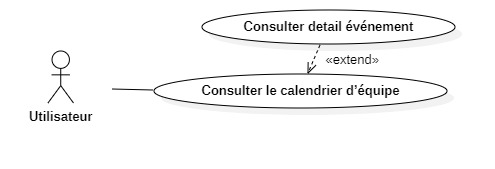
\includegraphics[width=11cm]{images/ccaleq.jpg}}
        \caption{Diagramme du cas d'utilisation <<Consulter le calendrier d’équipe>>}
        \label{fig:cal_equipe}
    \end{figure}
    \newpage
    \begin{table}[!ht]
        \vspace*{-1cm}
        \centering
        \caption{Description textuelle du Cas d’utilisation «Consulter le calendrier d’équipe»}
        \label{tab:consult_team_calendar}
        \renewcommand{\arraystretch}{1.2}
        \begin{tabular}{|p{4.2cm}|p{11cm}|}
        \hline
        \textbf{Cas d'utilisation} & Consulter le calendrier d’équipe \\
        \hline
        \textbf{Acteurs} & Utilisateur, Manager, RH \\
        \hline
        \textbf{Pré-conditions} & 
        \begin{itemize}
        \item Système en marche
        \item Acteur authentifié
        \item Données d’absences et d’autorisations enregistrées dans le système
        \end{itemize} \\
        \hline
        \textbf{Post-conditions} & L’acteur visualise les congés et autorisations de l’équipe dans un calendrier. \\
        \hline
        \textbf{Scénario de Base} & 
        \begin{enumerate}
        \item L’acteur accède à la section « Calendrier d’équipe »
        \item Le système affiche un calendrier avec les congés et autorisations de l’équipe
        \item Optionnel : L’acteur clique sur un événement pour voir les détails
        \end{enumerate} \\
        \hline
        \textbf{Exceptions} & 
        \begin{itemize}
        \item Aucune donnée disponible → Afficher « Aucun événement trouvé »
        \item Problème de chargement → Notification d’erreur technique
        \end{itemize} \\
        \hline
        \end{tabular}
    \end{table}

    \subsection{Raffinement du cas d'utilisation <<Consulter les tâches accomplies>>}
    La figure~\ref{fig:taches_accomplies} illustre le diagramme de cas d’utilisation « Consulter les tâches accomplies ».
    \begin{figure}[h]
        \centering
        \fbox{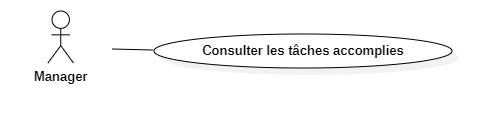
\includegraphics[width=10cm]{images/taches_accomplies.jpg}}
        \caption{Diagramme du cas d'utilisation <<Consulter les tâches accomplies>>}
        \label{fig:taches_accomplies}
    \end{figure}
\newpage
    \begin{table}[!ht]
        \vspace*{-1.2cm}
        \centering
        \caption{Description textuelle du Cas d’utilisation «Consulter les tâches accomplies»}
        \label{tab:consult_completed_tasks}
        \renewcommand{\arraystretch}{1.2}
        \begin{tabular}{|p{4.2cm}|p{11cm}|}
        \hline
        \textbf{Cas d'utilisation} & Consulter les tâches accomplies \\
        \hline
        \textbf{Acteurs} & Manager, RH \\
        \hline
        \textbf{Pré-conditions} & 
        \begin{itemize}
        \item Système en marche
        \item Acteur authentifié
        \item Tâches enregistrées et marquées comme accomplies
        \end{itemize} \\
        \hline
        \textbf{Post-conditions} & L’acteur visualise la liste des tâches accomplies par lui-même. \\
        \hline
        \textbf{Scénario de Base} & 
        \begin{enumerate}
        \item L’acteur accède à la section « Tâches accomplies »
        \item Le système affiche la liste des tâches marquées comme terminées
        \item L’acteur peut filtrer par période ou type de tâche
        \end{enumerate} \\
        \hline
        \textbf{Exceptions} & 
        \begin{itemize}
        \item Aucune tâche accomplie → Afficher « Aucune tâche trouvée »
        \item Erreur de chargement → Notification d’erreur technique
        \end{itemize} \\
        \hline
        \end{tabular}
    \end{table}
    \subsection{Raffinement du cas d'utilisation <<Consulter les rapports>>}
La figure~\ref{fig:rapports} illustre le diagramme de cas d’utilisation « Consulter les rapports ».
\begin{figure}[h]
    \centering
    \fbox{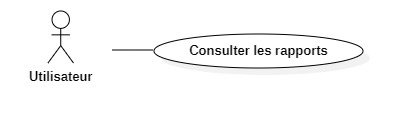
\includegraphics[width=10cm]{images/rapports.jpg}}
    \caption{Diagramme du cas d'utilisation <<Consulter les rapports>>}
    \label{fig:rapports}
\end{figure}
\newpage
\begin{table}[!ht]
    \centering
    \caption{Description textuelle du Cas d’utilisation «Consulter les rapports»}
    \label{tab:consult_reports}
    \renewcommand{\arraystretch}{1.2}
    \begin{tabular}{|p{4.2cm}|p{11cm}|}
    \hline
    \textbf{Cas d'utilisation} & Consulter les rapports \\
    \hline
    \textbf{Acteurs} & Utilisateur, Manager, RH \\
    \hline
    \textbf{Pré-conditions} & 
    \begin{itemize}
    \item Système en marche
    \item Acteur authentifié
    \item Données d’activités (ex. : congés) disponibles
    \end{itemize} \\
    \hline
    \textbf{Post-conditions} & L’acteur visualise un rapport d’activité généré. \\
    \hline
    \textbf{Scénario de Base} & 
    \begin{enumerate}
    \item L’acteur accède à la section « Mes congés » et clique sur la case « Générer un rapport »
    \item Le système génère un avis de congé
    \item Le rapport est affiché avec des graphiques
    \end{enumerate} \\
    \hline
    \textbf{Exceptions} & 
    \begin{itemize}
    \item Aucune donnée disponible → Afficher « Aucun rapport généré »
    \item Erreur de génération → Notification d’erreur technique
    \end{itemize} \\
    \hline
    \end{tabular}
\end{table}
\subsection{Raffinement du cas d'utilisation <<Implémentation d’un chatbot>>}
Le cas d’utilisation « Implémentation d’un chatbot » a pour objectif de fournir une assistance interactive aux administrateurs en intégrant un outil d’intelligence artificielle capable d’analyser et de présenter des statistiques sur les demandes traitées dans le système.\\
Pour ce faire, un modèle d’IA est téléchargé via Ollama, implémenté et intégré au backend à l’aide d’une API REST, puis entraîné sur les données des demandes pour générer des analyses pertinentes, comme le nombre de demandes approuvées ou rejetées par période.\\
Une interface web est ensuite créée et connectée au backend, permettant à l’administrateur d’interagir avec le chatbot pour obtenir des informations ou des actions assistées, améliorant ainsi l’efficacité de la gestion des processus administratifs.
\newpage
\begin{table}[!ht]
    \begin{adjustwidth}{-3.5cm}{-3.5cm}
    \vspace*{-2cm}
    \centering
    \caption{Description textuelle du Cas d’utilisation «Implémentation d’un chatbot»}
    \label{tab:implement_chatbot}
    \renewcommand{\arraystretch}{1.2}
    \begin{tabular}{|p{4.2cm}|p{11cm}|}
    \hline
    \textbf{Cas d'utilisation} & Implémentation d’un chatbot \\
    \hline
    \textbf{Acteurs} & Administrateur \\
    \hline
    \textbf{Pré-conditions} & 
    \begin{itemize}
    \item Système en marche
    \item Administrateur authentifié
    \item Serveur Ollama en marche
    \item Backend opérationnel avec une API pour intégrer le chatbot
    \end{itemize} \\
    \hline
    \textbf{Post-conditions} & 
    \begin{itemize}
    \item Le chatbot est intégré au backend et le backend à l’interface web
    \item Le chatbot fournit des statistiques sur les demandes (ex. : nombre de demandes approuvées/rejetées par période)
    \item L’administrateur interagit avec le chatbot via une interface web pour obtenir des informations ou des actions assistées
    \end{itemize} \\
    \hline
    \textbf{Scénario de Base} & 
    \begin{enumerate}
    \item L’équipe met en place un modèle d’IA adapté via Ollama de traitement du langage naturel comme LLaMA
    \item Le modèle est implémenté dans l’environnement du backend et intégré via une API REST pour communiquer avec le modèle Ollama
    \item Le modèle est entraîné avec les données des demandes pour fournir des statistiques (ex. : analyse du nombre de demandes par statut ou période)
    \item Une interface web front-end est développée pour permettre à l’administrateur d’interagir avec le chatbot
    \item L’interface web est intégrée avec le backend via des appels API pour envoyer les requêtes de l’administrateur et afficher les réponses du chatbot
    \item L’administrateur ouvre l’interface du chatbot dans l’application
    \item L’administrateur pose une question (ex. : « Quelles sont les statistiques des demandes ce mois-ci ? »)
    \item Le chatbot analyse la demande, interroge les données via le backend, et répond avec des statistiques (ex. : « 20 demandes approuvées, 5 rejetées »)
    \item Optionnel : Le chatbot propose des actions (ex. : « Voulez-vous exporter ces données ? »)
    \end{enumerate} \\
    \hline
    \textbf{Exceptions} & 
    \begin{itemize}
    \item Erreur de connexion entre front-end et backend → Message « Échec de communication avec le serveur »
    \item Demande incomprise par le chatbot → Réponse générique « Veuillez reformuler votre demande »
    \end{itemize} \\
    \hline
    \end{tabular}
\end{adjustwidth}
\end{table}
\clearpage
\section{Conception}
Dans cette partie, nous allons détailler la conception des cas d’utilisation du Sprint 4, dédié à l’analyse et aux améliorations, à travers un diagramme de classe global de ce sprint, suivi des diagrammes de classes et des diagrammes de séquences spécifiques au cas d’utilisation, afin de modéliser les interactions et les structures nécessaires à leur réalisation.
\subsection{Diagramme de classe du sprint 4}
La figure~\ref{fig:class_diagram_sprint4} illustre le diagramme de classe du Sprint 4.\\
\begin{figure}[h]
    \centering
    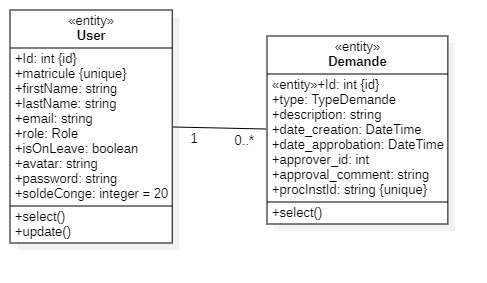
\includegraphics[width=15cm]{images/classprint4.jpg}
    \caption{Diagramme de classe du Sprint 4}
    \label{fig:class_diagram_sprint4}
\end{figure}
Le diagramme de classe est formé de :
\begin{itemize}
    \item \textbf{Classe "Demande"} : Gère les demandes soumises par les utilisateurs, comme les congés ou autorisations.
    \item \textbf{Classe "User"} : C’est la classe qui représente tous les utilisateurs ayant accès à la plateforme.
\end{itemize}
\subsection{Conception du Cas d'Utilisation «Consulter le calendrier d’équipe»}
La figure~\ref{fig:class_manage_calendar_equip} illustre le diagramme de classe du cas d’utilisation « Consulter le calendrier d’équipe ».
\newpage
\subsubsection{Diagramme de Classe}
\begin{figure}[h]
     \centering
     \fbox{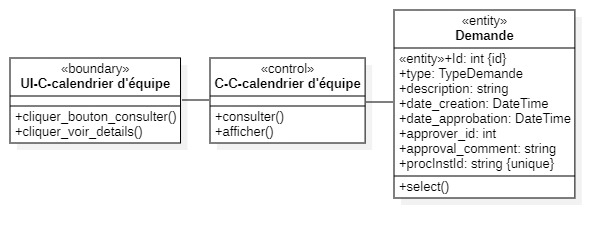
\includegraphics[width=12cm]{images/C_caleq.jpg}}
     \caption{Diagramme de classe du cas d'utilisation <<Consulter le calendrier d’équipe>>}
     \label{fig:class_manage_calendar_equip}
\end{figure}
\subsubsection{Diagramme de Séquence}
L’utilisateur se connecte, accède à la section « Calendrier d’équipe », consulte les événements (congés et autorisations) de son équipe, clique sur un événement, et visualise les détails tels que la date de début et la date de fin. Ce scénario est modélisé dans la figure~\ref{fig:seq_manage_calendar_equip}.
\begin{figure}[h]
    \centering
    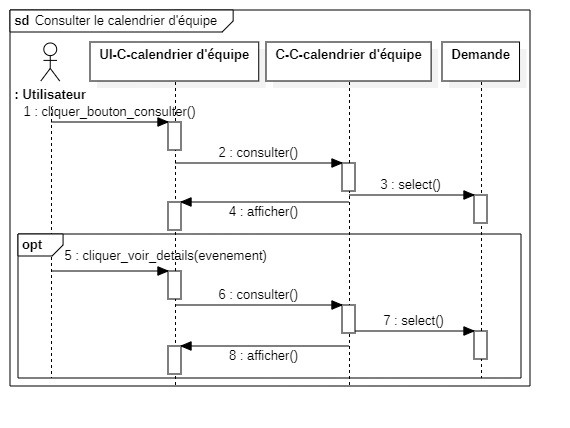
\includegraphics[width=13cm]{images/S_caleq.jpg}
    \caption{Diagramme de séquence du cas d'utilisation <<Consulter le calendrier d’équipe>>}
    \label{fig:seq_manage_calendar_equip}
\end{figure}
\newpage
\subsection{Conception du Cas d'Utilisation «Consulter les tâches accomplies»}
La figure~\ref{fig:class_completed_tasks} illustre le diagramme de classe du cas d’utilisation « Consulter les tâches accomplies ».
\subsubsection{Diagramme de Classe}
\begin{figure}[h]
     \centering
     \fbox{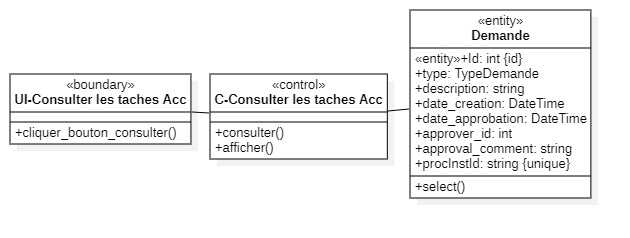
\includegraphics[width=12cm]{images/C_taches_accomplies.jpg}}
     \caption{Diagramme de classe du cas d'utilisation <<Consulter les tâches accomplies>>}
     \label{fig:class_completed_tasks}
\end{figure}
\subsubsection{Diagramme de Séquence}
Le manager ou RH se connecte, accède à la section « Tâches accomplies », consulte la liste des tâches qu’il a réalisées organisés par période. Ce scénario est modélisé dans la figure~\ref{fig:seq_completed_tasks}.
\begin{figure}[h]
    \centering
    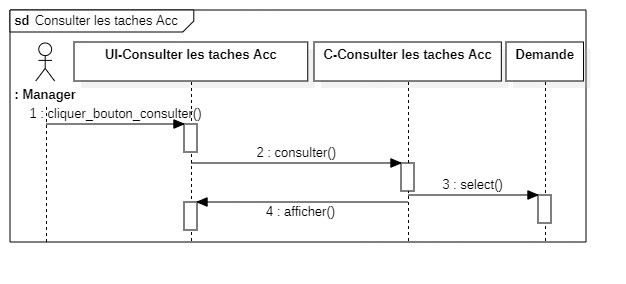
\includegraphics[width=13cm]{images/S_taches_accomplies.jpg}
    \caption{Diagramme de séquence du cas d'utilisation <<Consulter les tâches accomplies>>}
    \label{fig:seq_completed_tasks}
\end{figure}
\subsection{Conception du Cas d'Utilisation «Consulter les rapports»}
La figure~\ref{fig:class_consult_reports} illustre le diagramme de classe du cas d’utilisation « Consulter les rapports ».
\newpage
\subsubsection{Diagramme de Classe}
\begin{figure}[h]
     \centering
     \fbox{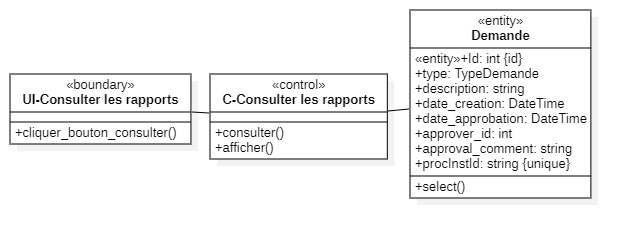
\includegraphics[width=12cm]{images/C_rapports.jpg}}
     \caption{Diagramme de classe du cas d'utilisation <<Consulter les rapports>>}
     \label{fig:class_consult_reports}
\end{figure}
\subsubsection{Diagramme de Séquence}
L’utilisateur, manager ou RH se connecte, accède à la section « Rapports », sélectionne un type de rapport (ex. : congés), choisit une période, et visualise le rapport généré sous forme de tableaux ou graphiques. Ce scénario est modélisé dans la figure~\ref{fig:seq_consult_reports}.
\begin{figure}[h]
    \centering
    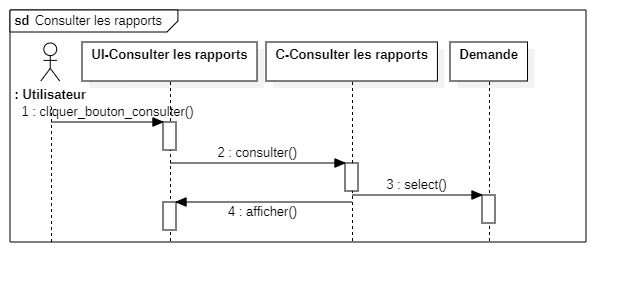
\includegraphics[width=13cm]{images/S_rapports.jpg}
    \caption{Diagramme de séquence du cas d'utilisation <<Consulter les rapports>>}
    \label{fig:seq_consult_reports}
\end{figure}
\subsection{Conception du Cas d'Utilisation «Implémentation d’un chatbot»}
La figure~\ref{fig:class_implement_chatbot} illustre le diagramme de classe du cas d’utilisation « Implémentation d’un chatbot ».
\newpage
\subsubsection{Diagramme de Classe}
\begin{figure}[h]
     \centering
     \fbox{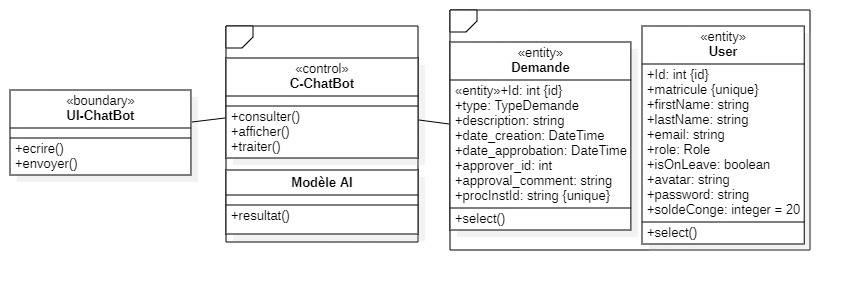
\includegraphics[width=12cm]{images/S_chatbot.jpg}}
     \caption{Diagramme de classe du cas d'utilisation <<Implémentation d’un chatbot>>}
     \label{fig:class_implement_chatbot}
\end{figure}
\subsubsection{Diagramme de Séquence}
L’administrateur se connecte, ouvre l’interface du chatbot, pose une question (ex. : « Quelles sont les statistiques des congés ce mois-ci ? »), le modèle d’IA, qui connaît l’architecture des tables sauf « Demande » et « User », traduit cette interrogation en une requête SQL (ex. : \texttt{SELECT COUNT(*) FROM DEMANDE WHERE MONTH(date\_debut) = 6}), l’envoie au contrôleur, qui exécute la requête et renvoie le résultat (ex. : « 15 congés ce mois-ci ») à la vue pour affichage.
\begin{figure}[h]
    \centering
    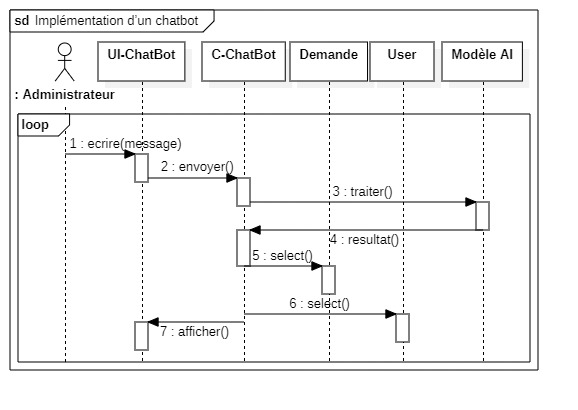
\includegraphics[width=13cm]{images/C_chatbot.jpg}
    \caption{Diagramme de séquence du cas d'utilisation <<Implémentation d’un chatbot>>}
    \label{fig:seq_implement_chatbot}
\end{figure}
\section{Réalisation}
\subsection{Consulter le calendrier d’équipe}
Les figure~\ref{fig:team_calendar} et \ref{fig:team_calendar1} présentent les interfaces permettant aux utilisateurs, managers et RH de consulter les événements de leur équipe, ainsi que les détails de ces événements. \\
\begin{figure}[h]
    \centering
    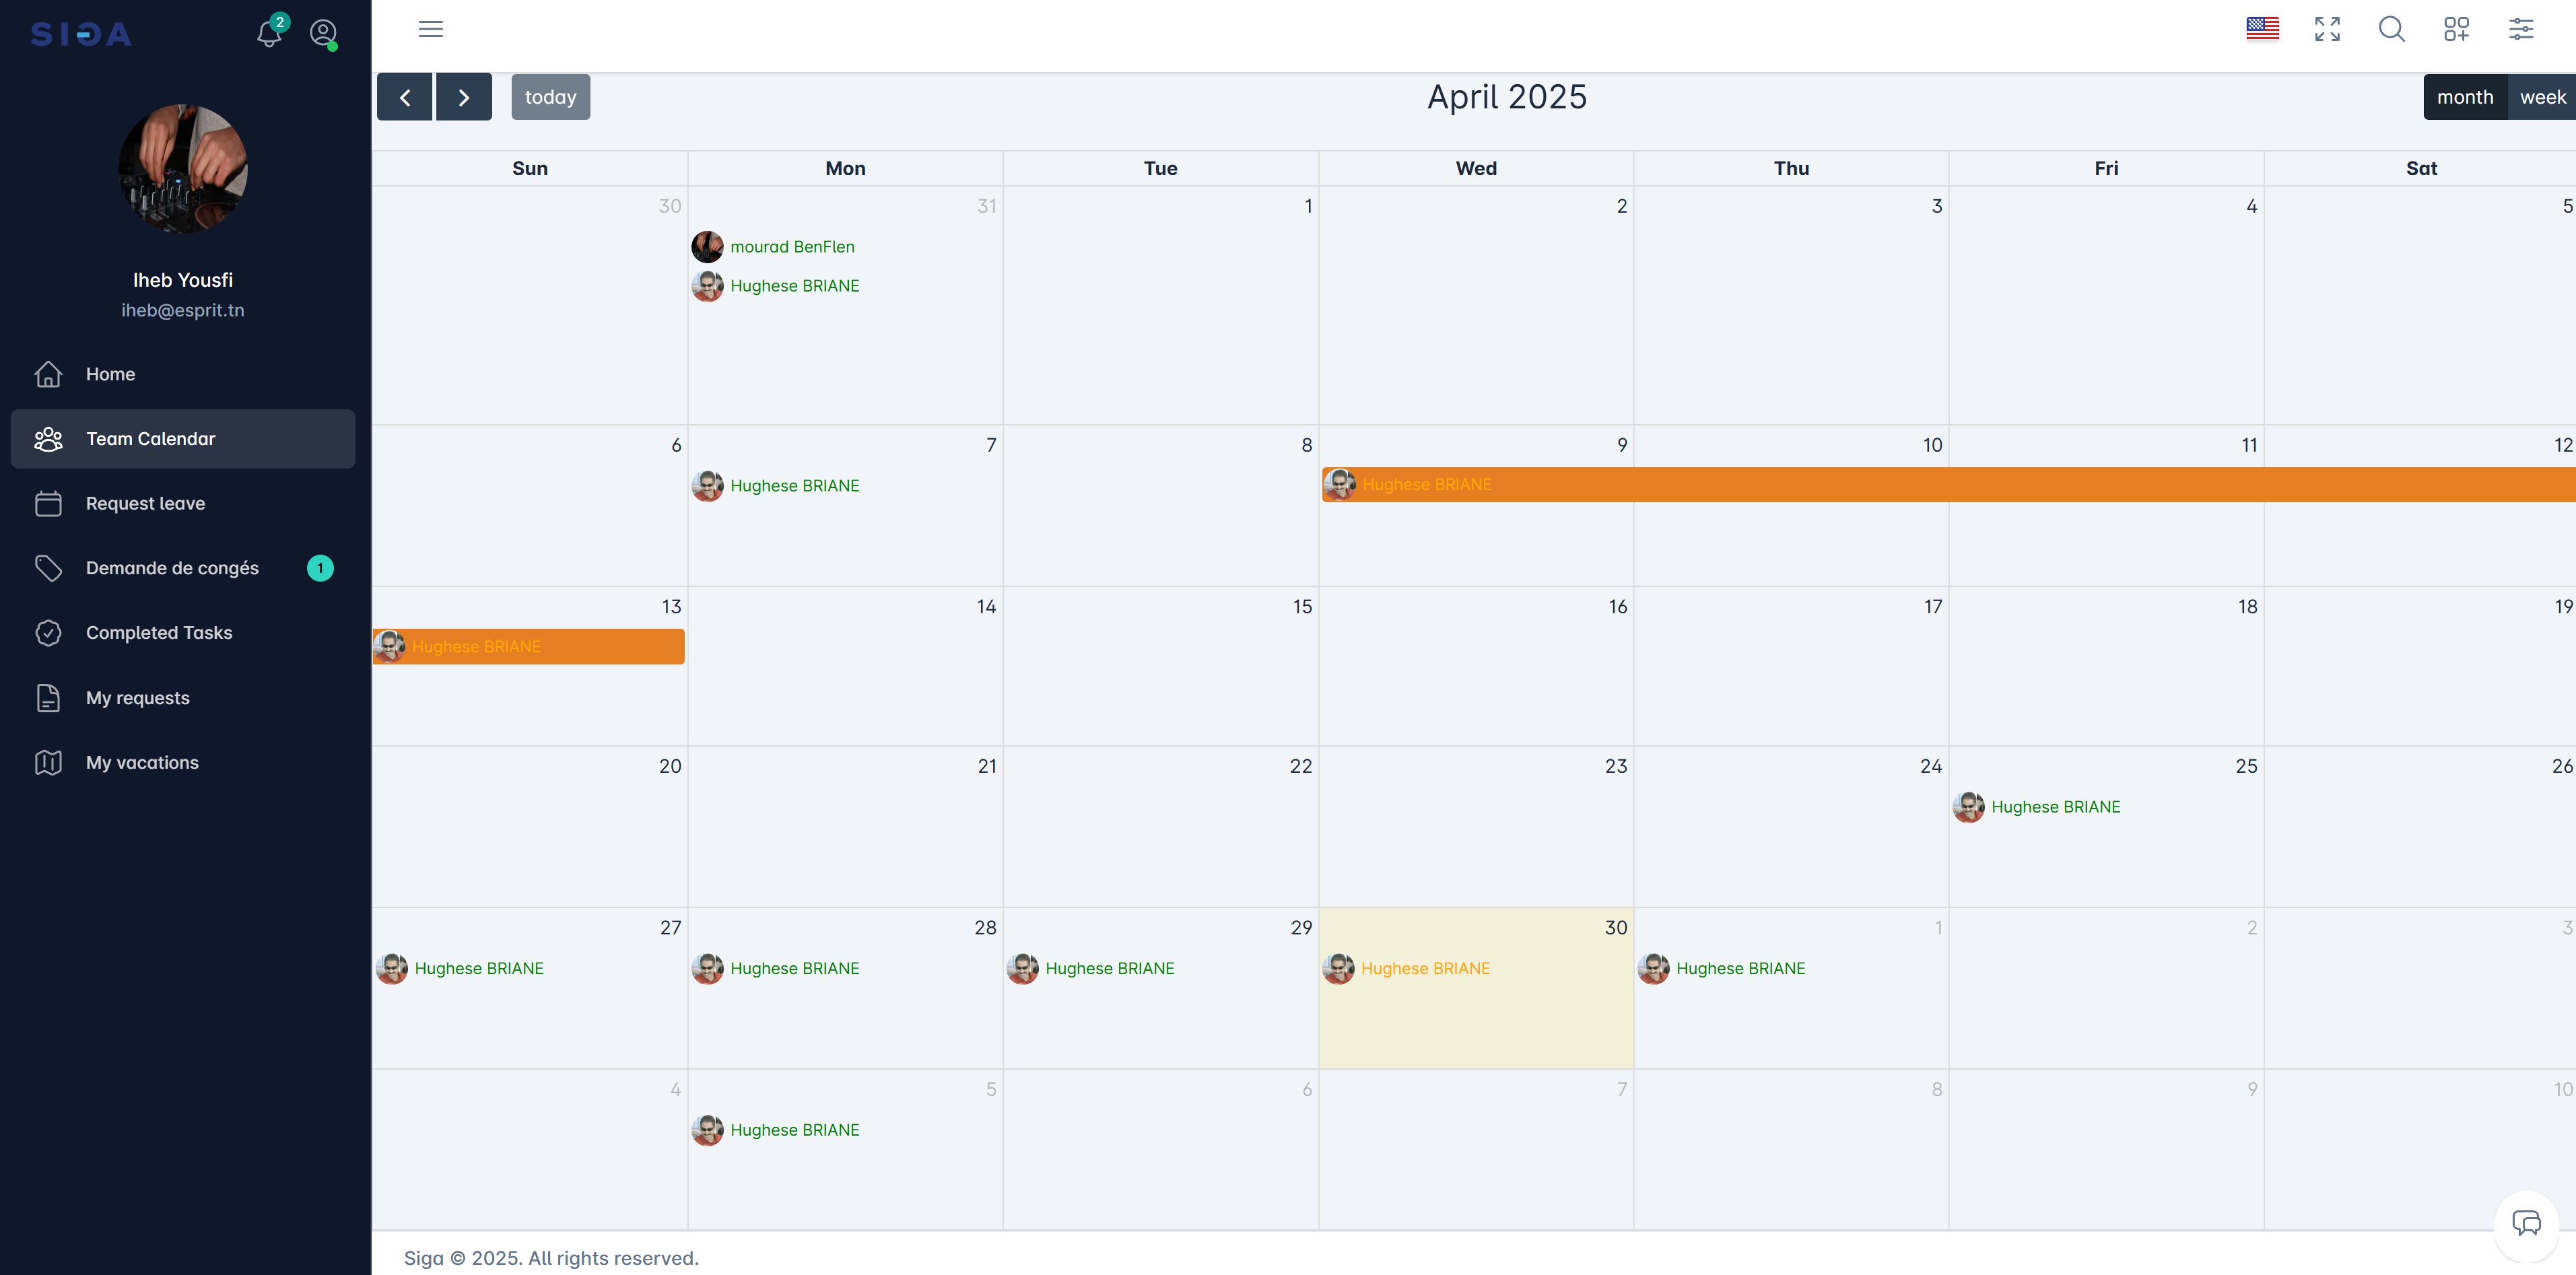
\includegraphics[width=15cm]{images/realisation/team_calendar.png}
    \caption{Interface du cas d'utilisation «Consulter le calendrier d’équipe»}
    \label{fig:team_calendar}
\end{figure}
\begin{figure}[h]
    \centering
    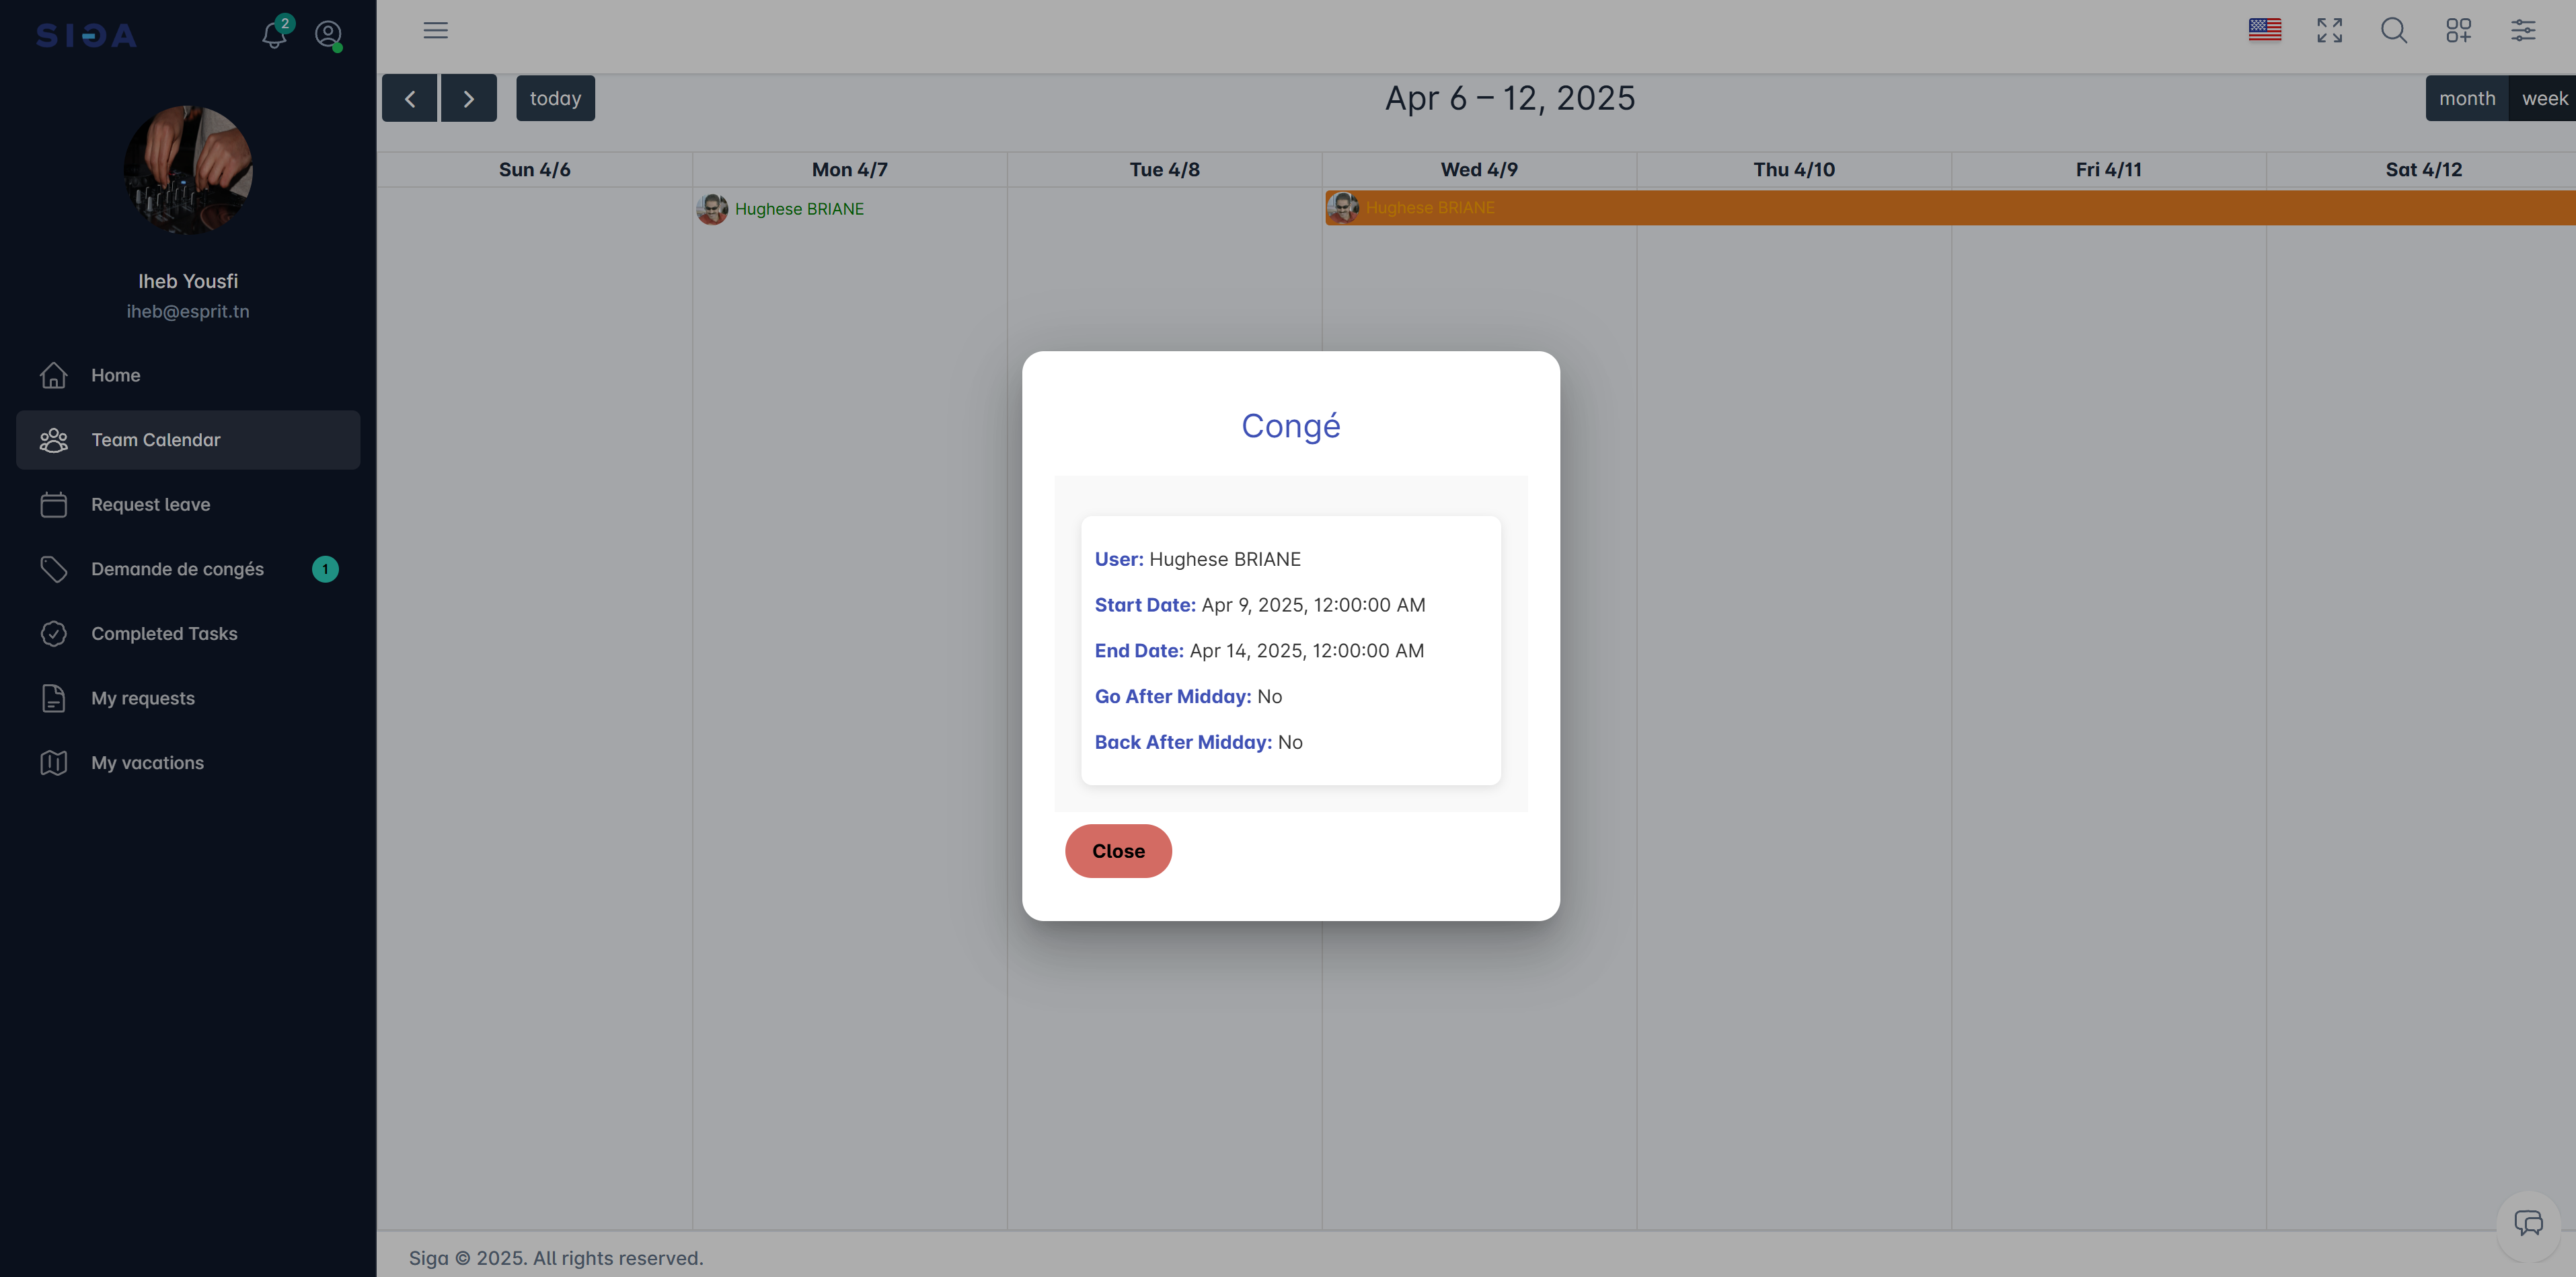
\includegraphics[width=15cm]{images/realisation/team_calendar2.png}
    \caption{Interface du cas d'utilisation «Consulter le calendrier d’équipe (voir details)»}
    \label{fig:team_calendar1}
\end{figure}
\clearpage
\subsection{Consulter les tâches accomplies}
La figure~\ref{fig:completed_tasks} illustre l’interface permettant aux managers et RH de suivre leurs tâches réalisées. \\
\begin{figure}[h]
    \centering
    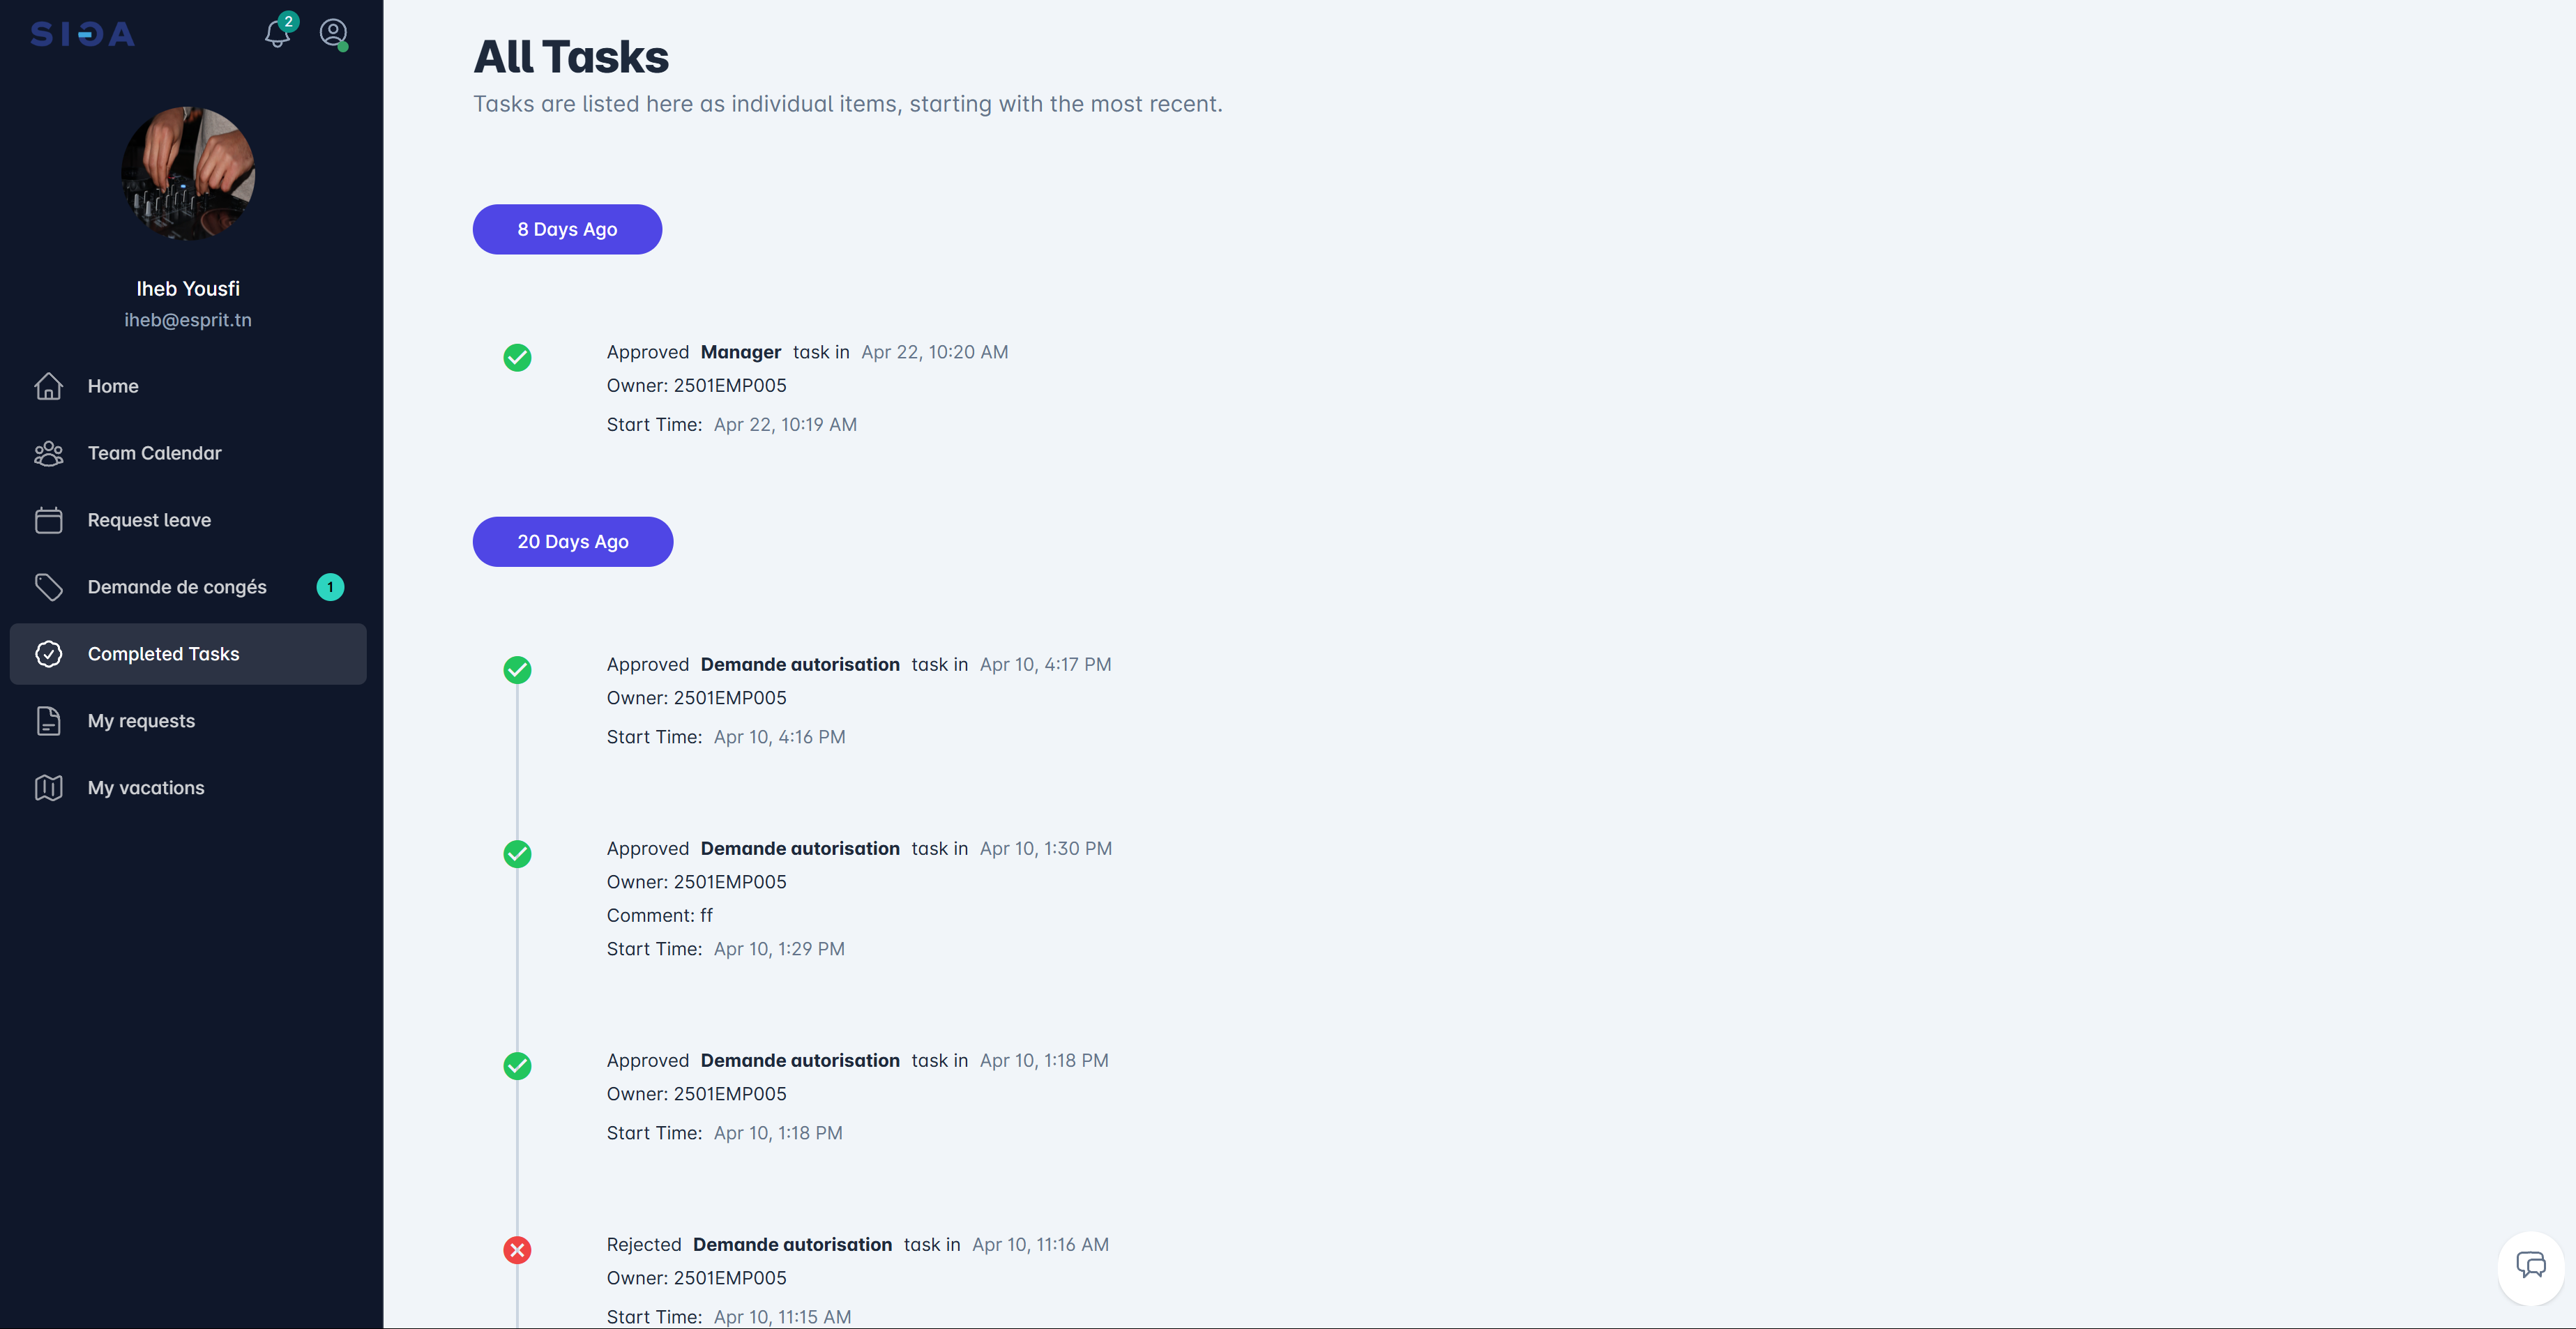
\includegraphics[width=14cm]{images/realisation/completed_tasks.png}
    \caption{Interface du cas d'utilisation «Consulter les tâches accomplies»}
    \label{fig:completed_tasks}
\end{figure}
\subsection{Consulter les rapports}
Les figure~\ref{fig:consult_reports} et \ref{fig:consult_reports1} présentent les interfaces de consultation des rapports, accessible aux utilisateurs, managers et RH. \\
\begin{figure}[h]
    \centering
    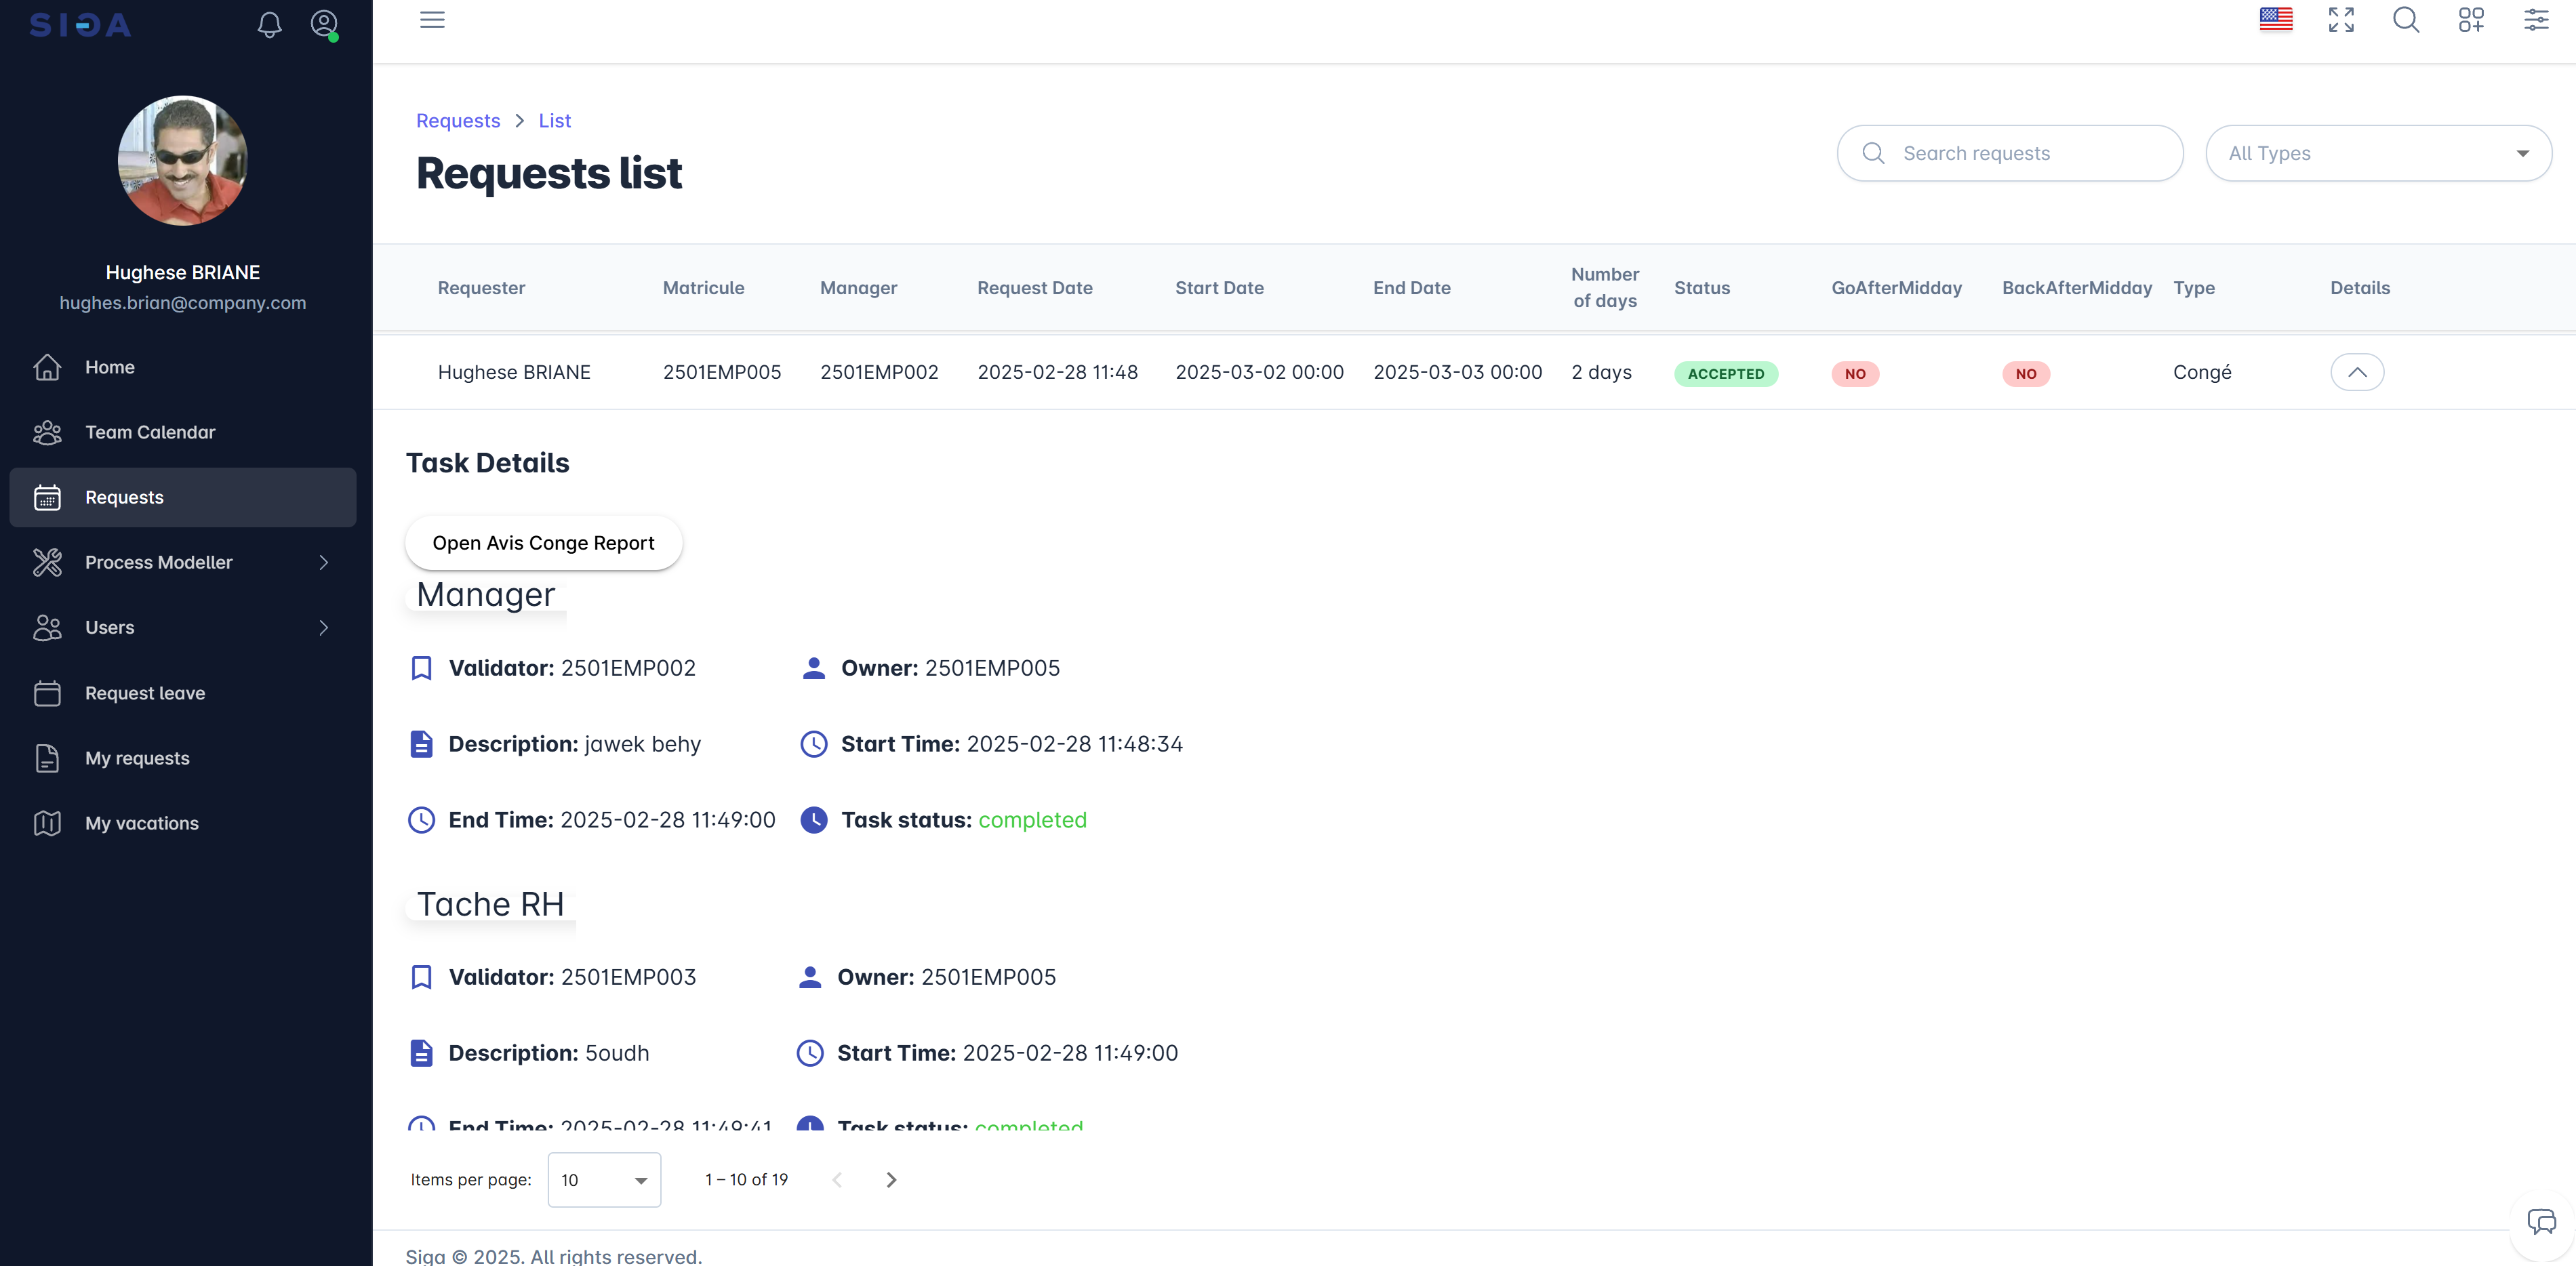
\includegraphics[width=14cm]{images/realisation/consult_reports.png}
    \caption{Interface du cas d'utilisation «Consulter les rapports»}
    \label{fig:consult_reports}
\end{figure}
\begin{figure}[h]
    \centering
    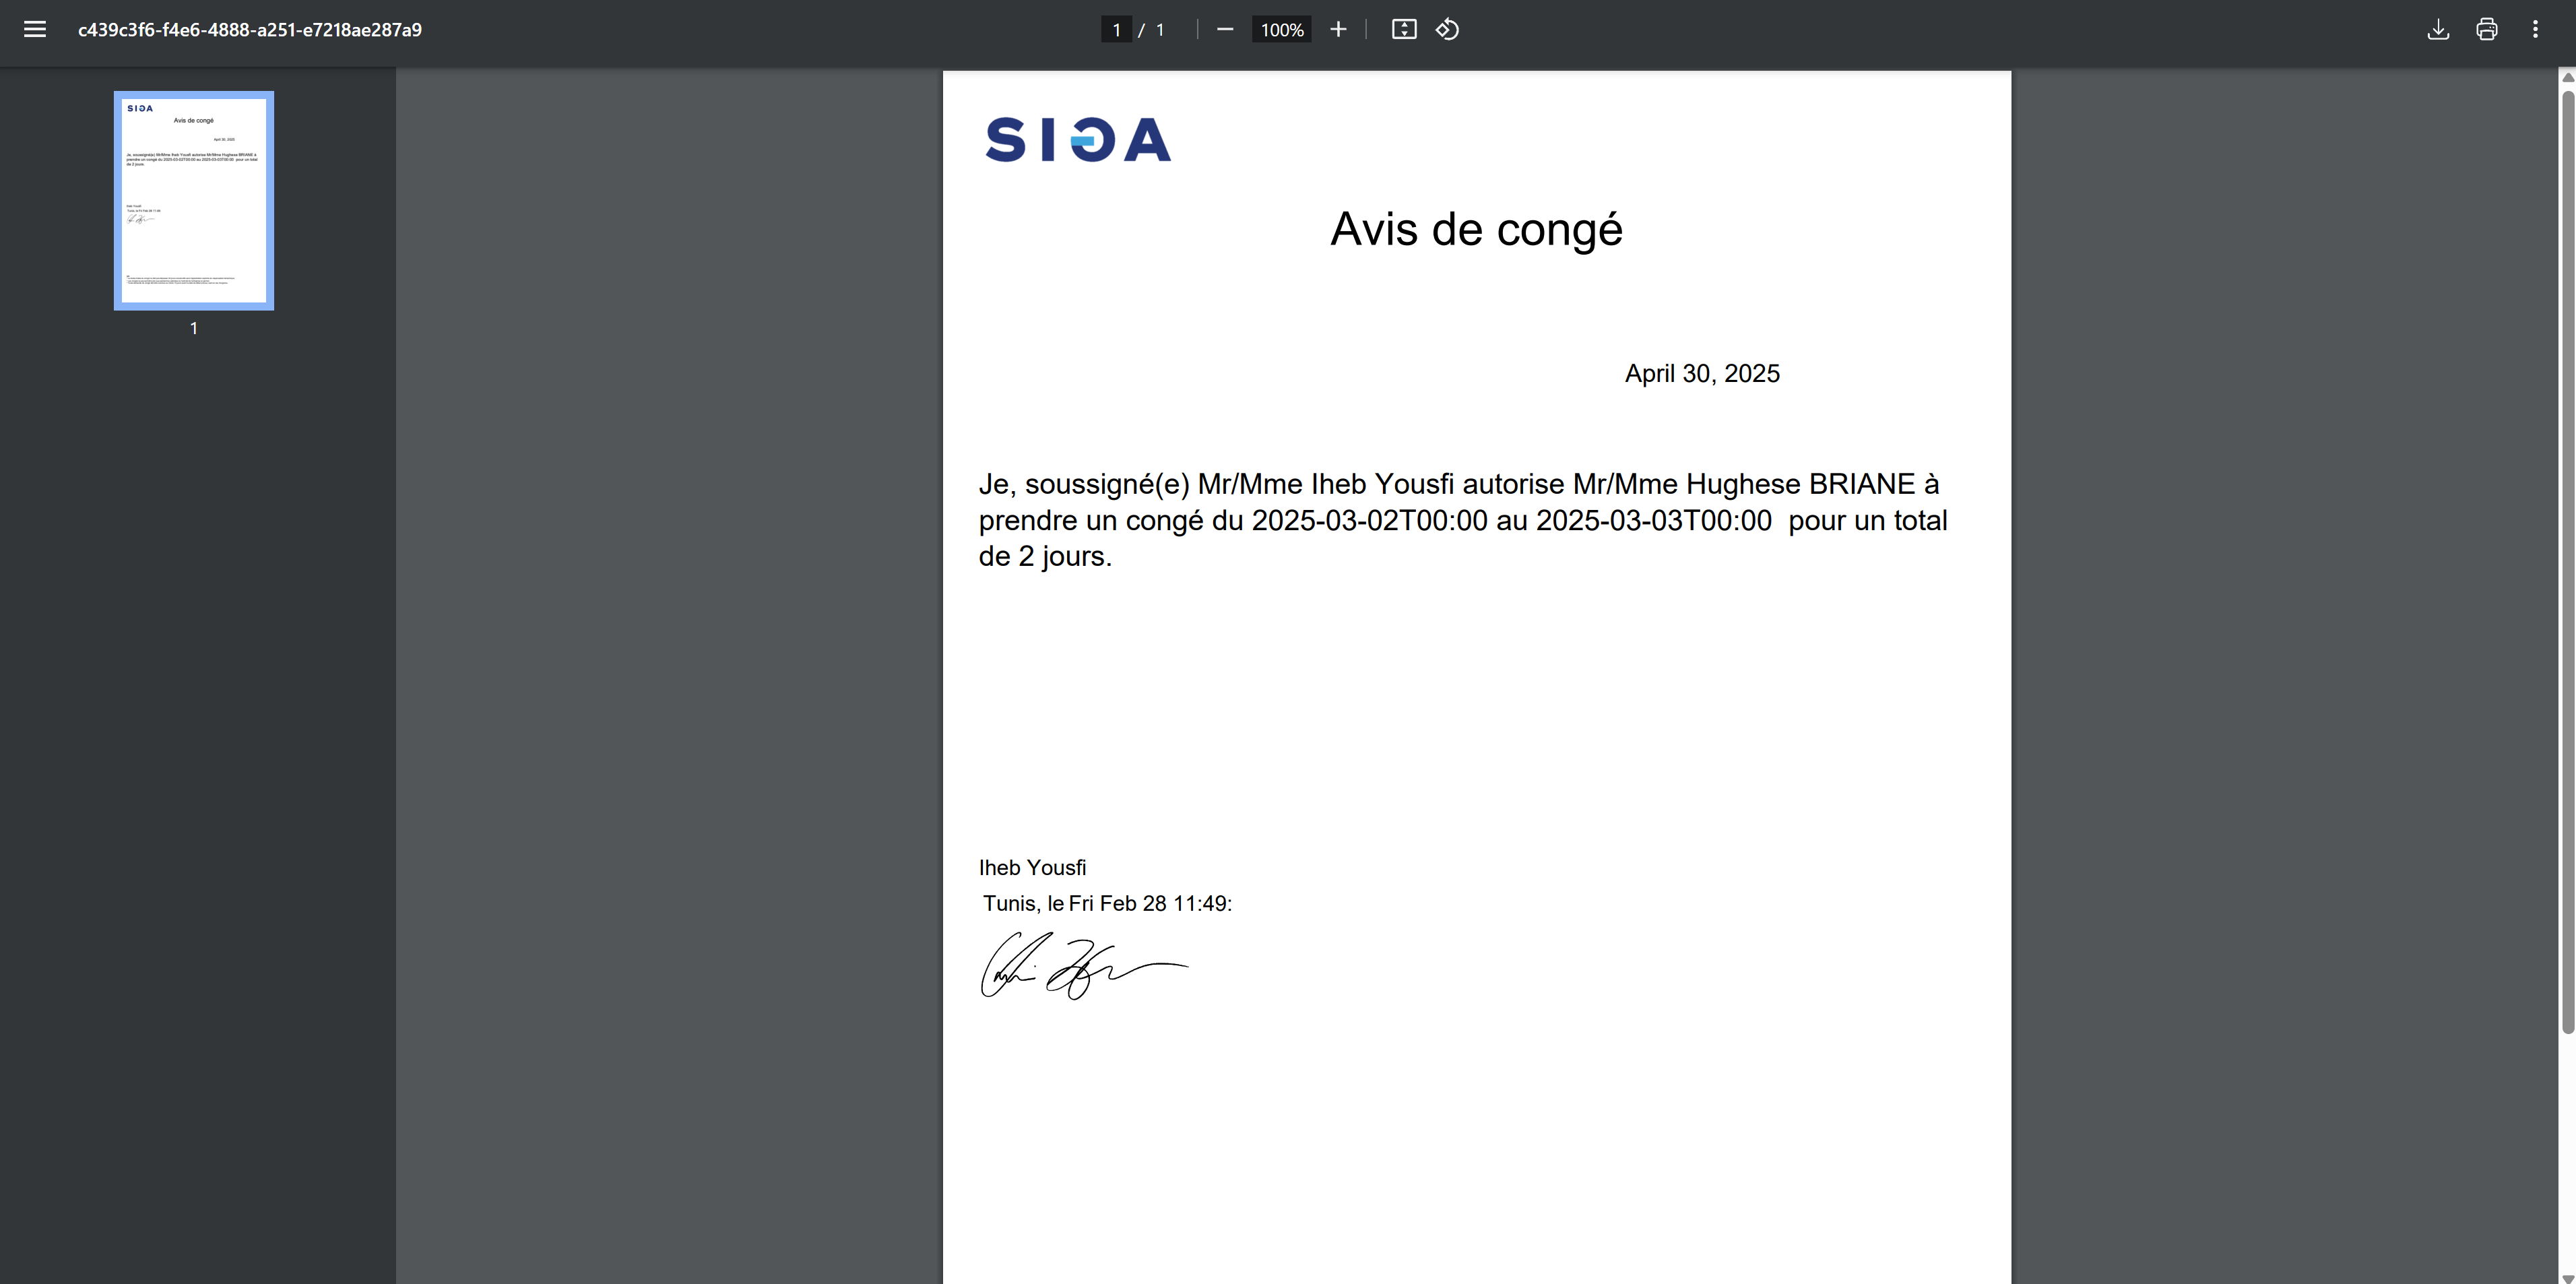
\includegraphics[width=16cm]{images/realisation/consult_reports1.png}
    \caption{Interface du cas d'utilisation «Consulter les rapports»}
    \label{fig:consult_reports1}
\end{figure}
\subsection{Implémentation d’un chatbot}
Les figure~\ref{fig:chatbot_interface}, \ref{fig:chatbot_interface1} et \ref{fig:chatbot_interface2} présentent l'implementation et l’interface du chatbot intégré pour assister les administrateurs. \\
\textbf{Scénario utilisateur} : 
\begin{enumerate}
    \item L’administrateur se connecte à son espace
    \item Il ouvre l’interface du chatbot via un bouton dédié
    \item Le système affiche une fenêtre de discussion où :
    \begin{itemize}
        \item L’administrateur peut poser des questions (ex. : « Statistiques des congés ce mois-ci ? »)
        \item Le chatbot répond avec des données (ex. : « 15 congés ce mois-ci »)
        \item Optionnel : insertion directe des requétes SQL
    \end{itemize}
\end{enumerate}
\begin{figure}[h]
    \centering
    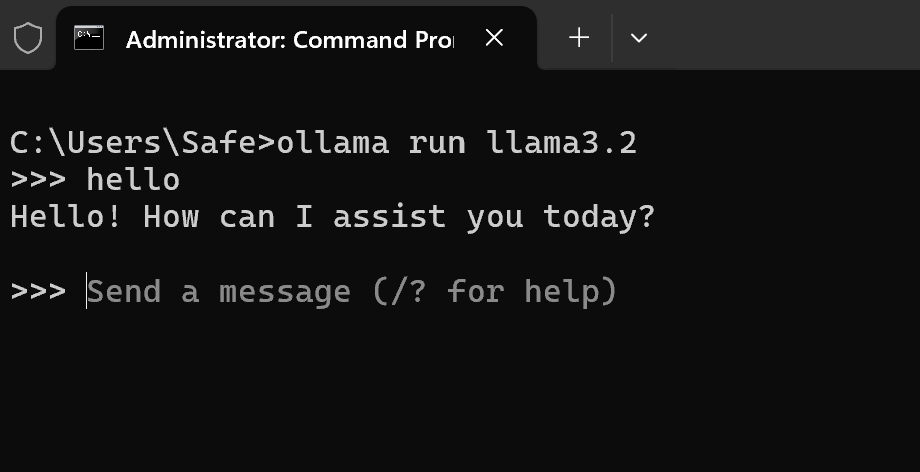
\includegraphics[width=16cm]{images/realisation/ollama.png}
    \caption{Interface du cas d'utilisation «Implémentation d’un chatbot»}
    \label{fig:chatbot_interface}
\end{figure}
\begin{figure}[h]
    \centering
    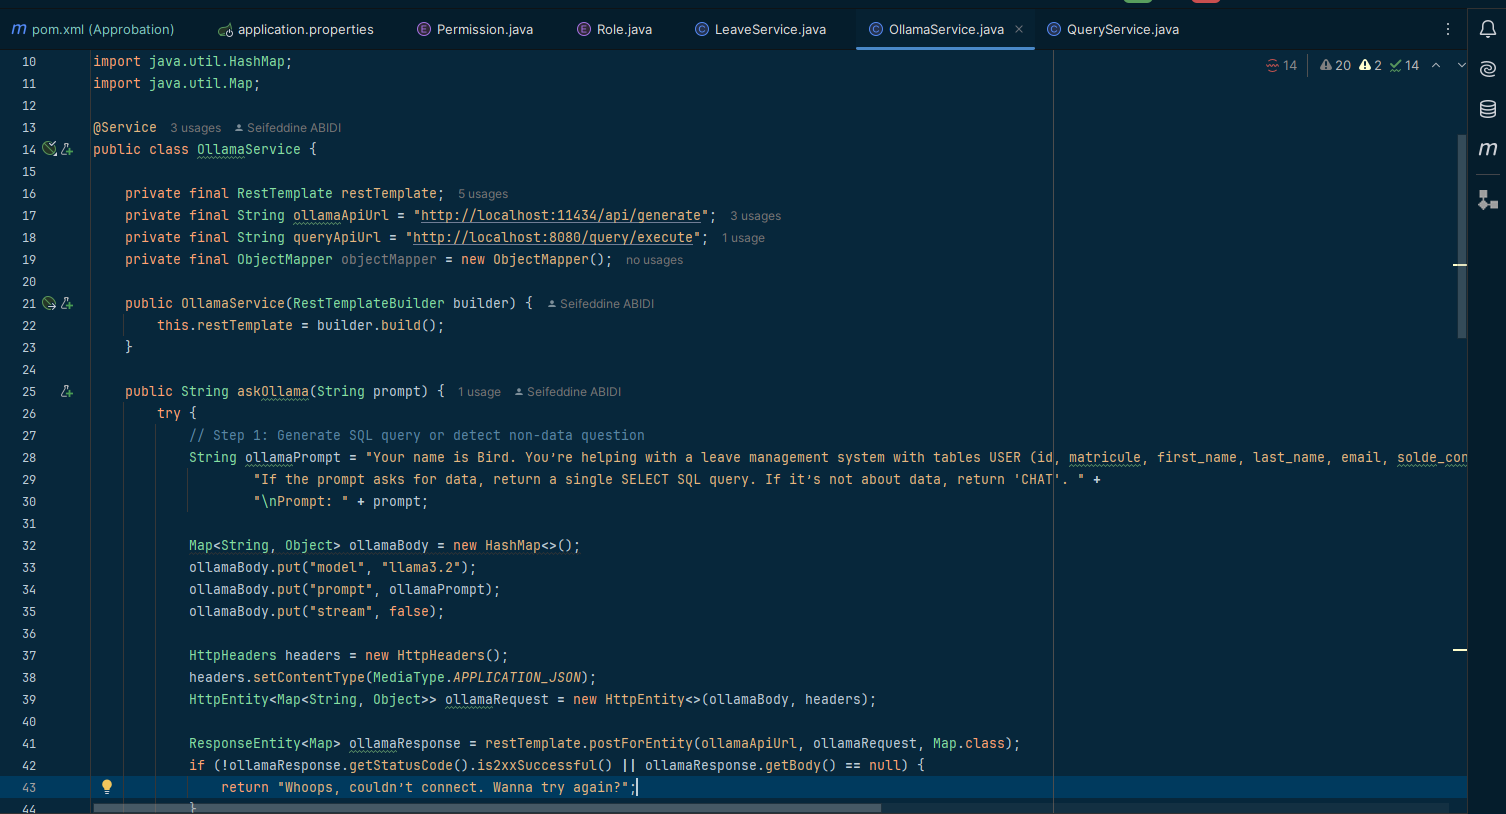
\includegraphics[width=16cm]{images/realisation/ollama2.png}
    \caption{Interface du cas d'utilisation «Implémentation d’un chatbot»}
    \label{fig:chatbot_interface1}
\end{figure}
\clearpage
\begin{figure}[h]
    \centering
    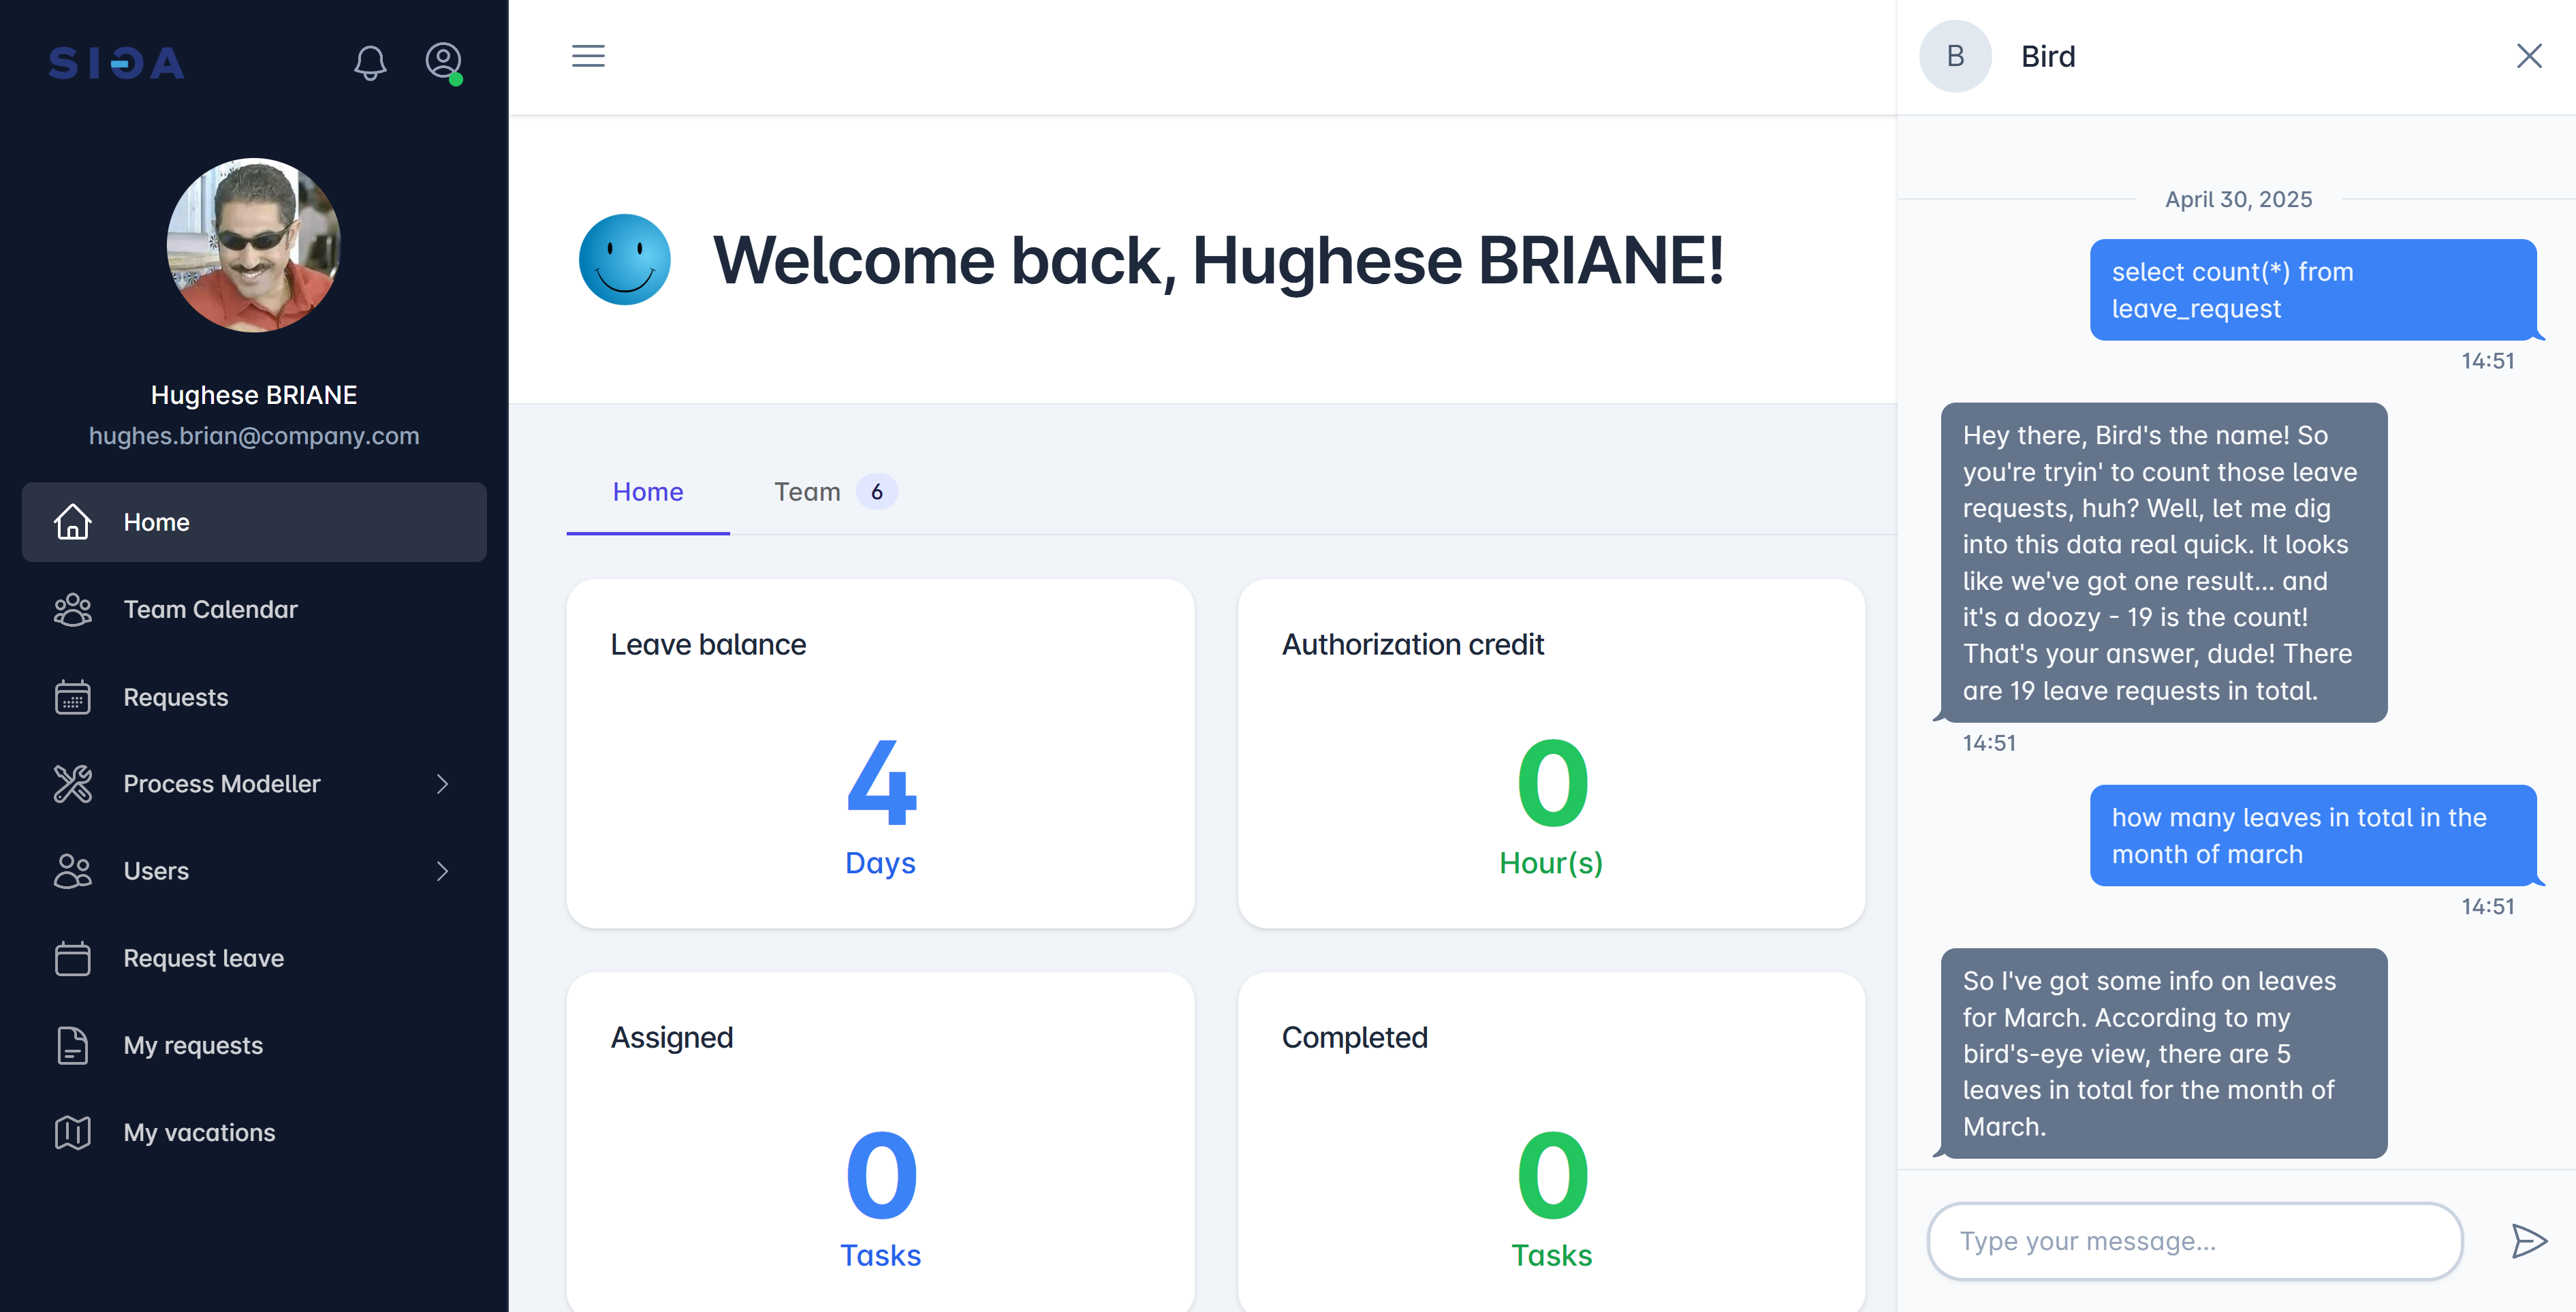
\includegraphics[width=16cm]{images/realisation/ollama3.png}
    \caption{Interface du cas d'utilisation «Implémentation d’un chatbot»}
    \label{fig:chatbot_interface2}
\end{figure}
\section{Conclusion}
Le Sprint 4 a permis de consolider les avancées des sprints précédents en introduisant des outils d’analyse et des améliorations significatives pour optimiser l’expérience utilisateur au sein de la plateforme.\\
Les fonctionnalités développées, telles que la consultation du calendrier d’équipe, des tâches accomplies et des rapports d’activité, offrent aux utilisateurs, managers et RH une vision claire et structurée de leurs données, renforçant ainsi leur capacité à suivre et analyser les processus.\\
L’intégration d’un chatbot interactif pour les administrateurs marque une avancée notable en matière d’assistance, en fournissant des statistiques pertinentes via des requêtes SQL générées dynamiquement.\\
Grâce à une conception détaillée et une réalisation soignée, ce sprint a répondu aux besoins identifiés tout en ouvrant la voie à de futures évolutions pour encore plus d’interactivité et d’efficacité dans la gestion des ressources humaines.